\documentclass[twocolumn]{aastex62}

\newcommand{\vdag}{(v)^\dagger}
\newcommand\aastex{AAS\TeX}
\newcommand\latex{La\TeX}
\usepackage{amsmath}
\usepackage{physics}
\usepackage{hyperref}
\usepackage{natbib}
\usepackage[T1]{fontenc}
\usepackage[english]{babel}
\usepackage[utf8]{inputenc}
\usepackage{wasysym}

\begin{document}

\title{\Large AST5220-Milestone III: Evolution of structure in the Universe}

\author{Nils-Ole Stutzer}

\begin{abstract}
    
    \textit{The codes for this paper can be found at:} \newline \url{https://github.com/SagittariusA-Star/AST5220-Milestones}
\end{abstract}

\section{Introduction} \label{sec:Intro}

\section{Method} \label{sec:Method}

\begin{figure*}
    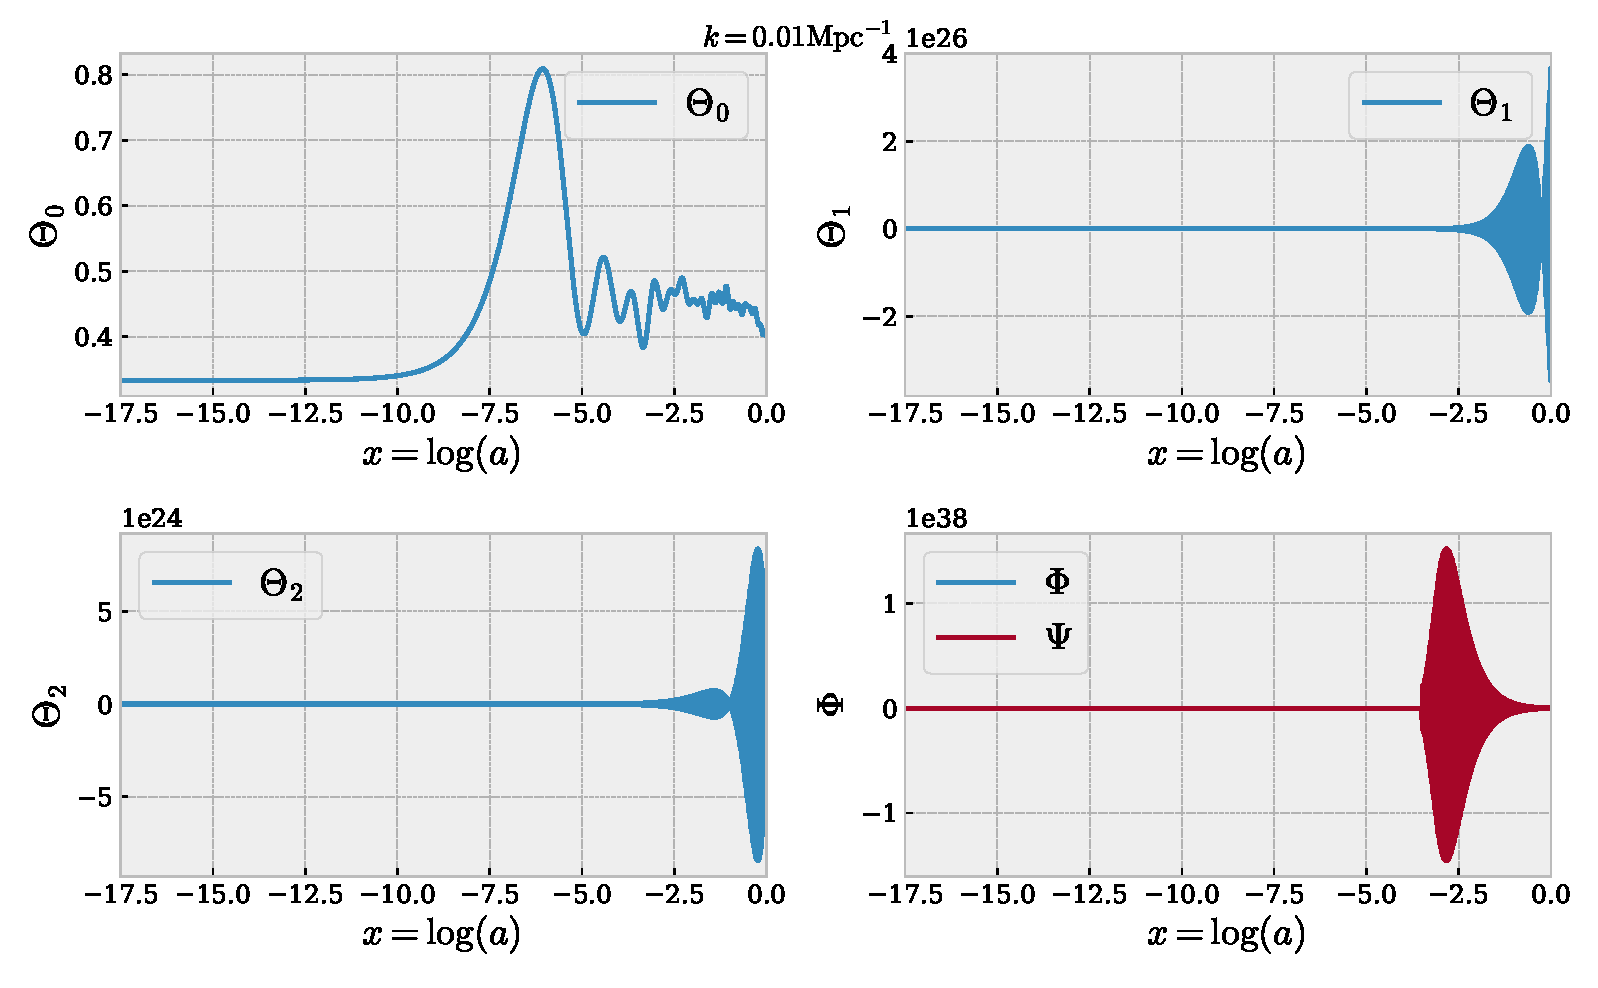
\includegraphics[scale = 0.65]{Figures/fig1.pdf}
    \caption{The figure shows (\textbf{Upper left}) the monopole moment $\Theta_0 = \frac{1}{4}\delta_\gamma$ and (\textbf{upper right}) the dipole moment $\Theta_1 = -\frac{1}{3}v_\gamma$, roughly corresponding to the density and velocity perturbation of radiation energy-density perturbation respectively. Also shown (\textbf{lower right}) are the metric perturbations $\Phi$ and $\Psi$ in the Newtonian gauge. All quantities plotted are functions of the log-scale factor $x = \ln a$ and scale $k$, and are shown for several different wavenumbers. The background color marks the epoch of dominance; yellow, blue and purple represent radiation, matter and dark energy dominated epochs respectively. The red background color corresponds to the epoch of recombination and the vertical red dotted line marks the precise time of recombination.} 
    \label{fig:fig1}
\end{figure*}

\begin{figure*}
    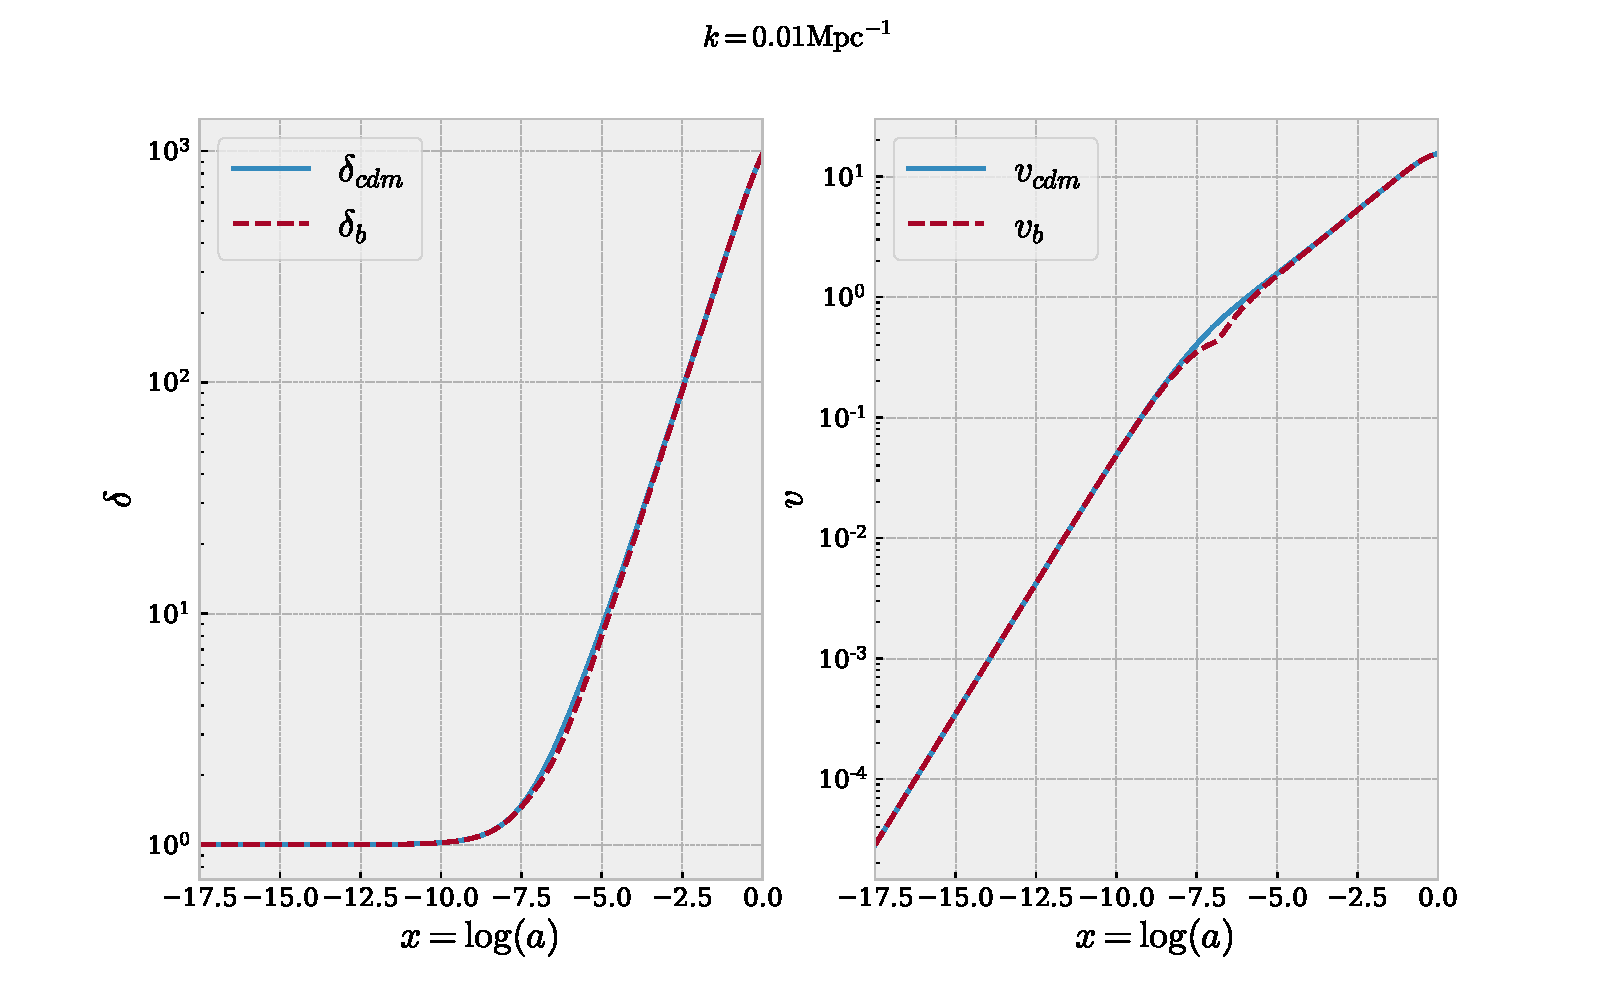
\includegraphics[scale = 0.65]{Figures/fig2.pdf}
    \caption{The left panel shows the density perturbations of the dark and baryonic matter perturbations (solid and dashed lines respectively). The right panel shows the velocity perturbations for dark and baryonic matter (same meaning of line style as in the left panel). The quantities shown are functions of the log-scale $x = \ln a$ and scale, and are plotted for several wavenumbers $k$.  The background color marks the epoch of dominance; yellow, blue and purple represent radiation, matter and dark energy dominated epochs respectively. The red background color corresponds to the epoch of recombination and the vertical red dotted line marks the precise time of recombination.}
    \label{fig:fig2}
\end{figure*}


\section{Results/Discussion}\label{sec:Results}

\section{Conclusion} \label{sec:Conclusion}

\newpage
\bibliography{ref}
\bibliographystyle{aasjournal}
\end{document}